\section{Japanese Grand prix}

\subsection{Circuit Analysis}

\textbf{Circuit Name:} Suzuka International Racing Course (Suzuka, Japan) \\
\textbf{Length:} 5.807 km - \textbf{Laps:} 53 - \textbf{Total Distance:} 307.471 km

\begin{figure}[H]
    \centering
    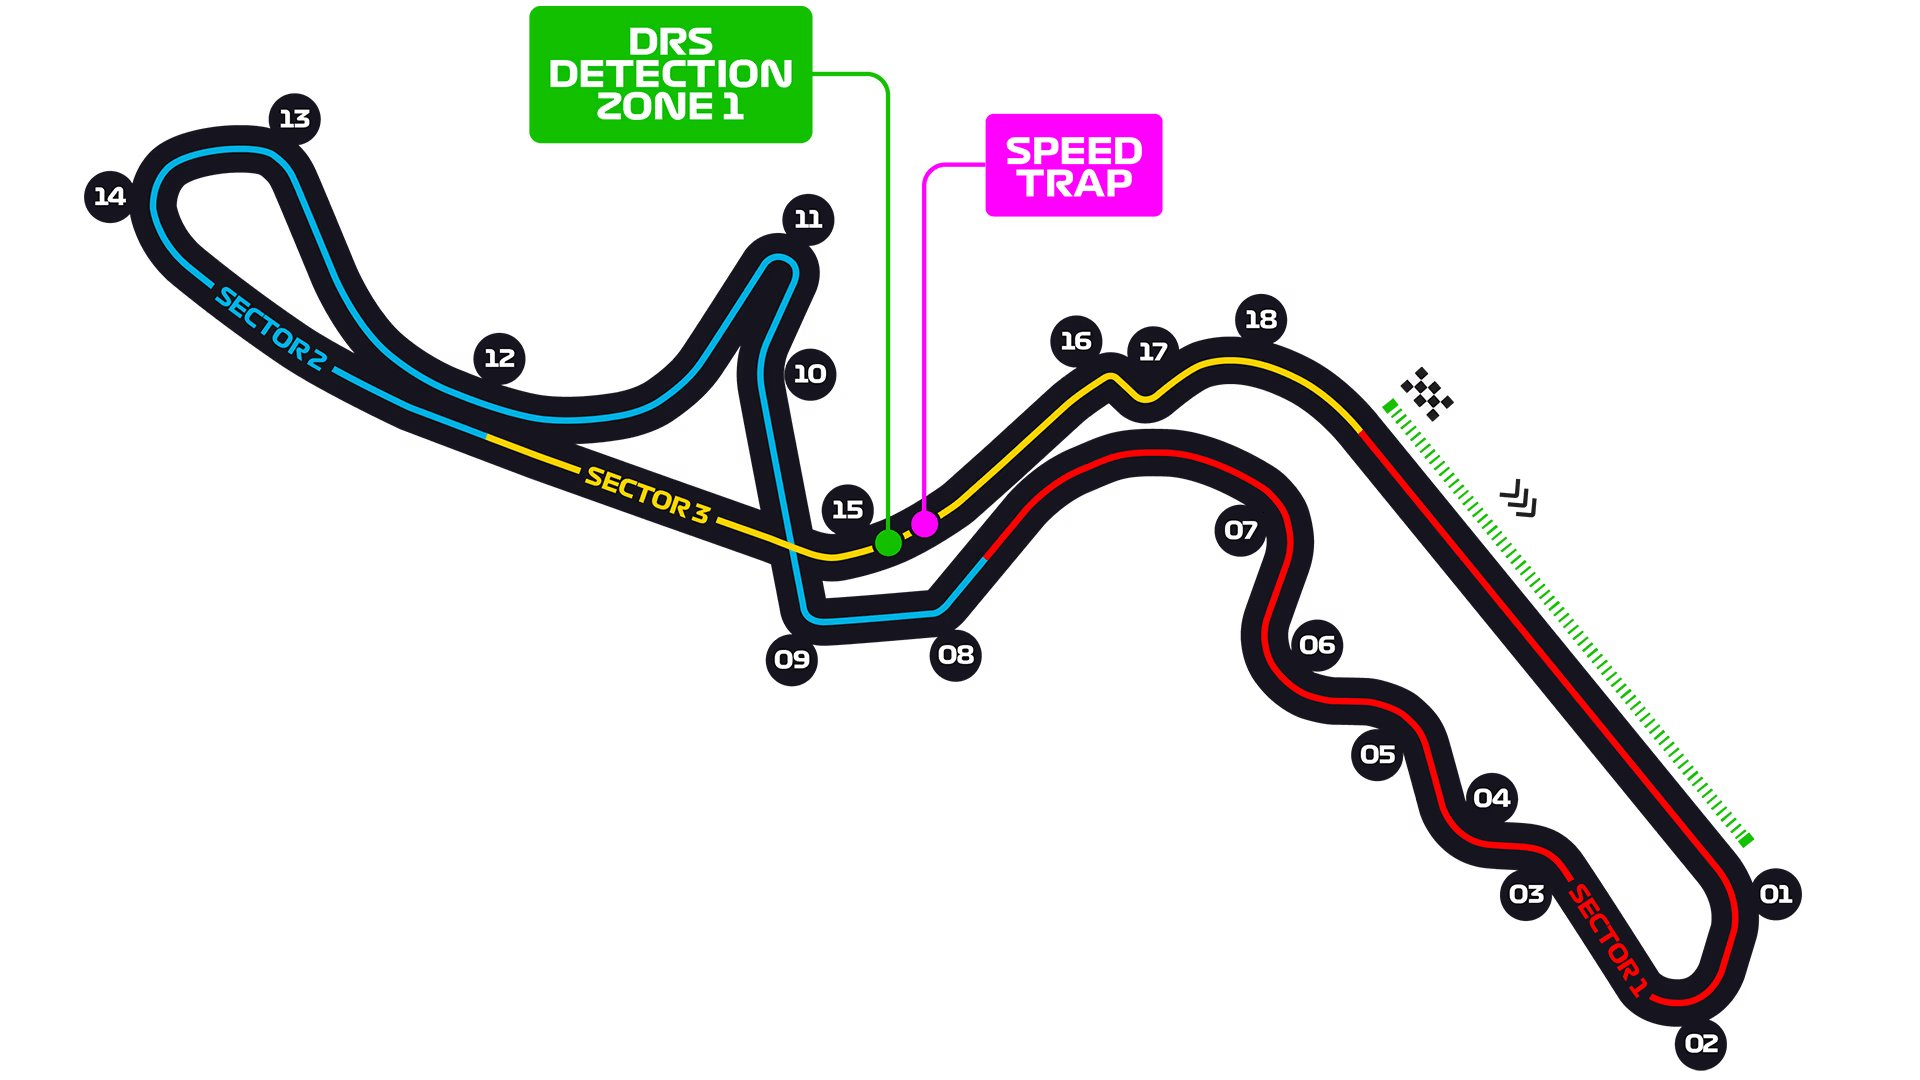
\includegraphics[width=0.75\linewidth]{images/4.Japan_Circuit.jpg}
\end{figure}

\begin{itemize}
    \item \textbf{Lap Record} : 1:28.877 (2023, Max Verstappen - Red Bull).
    
    \item \textbf{Number of Corners \& Key Features} : 18 turns (10 right, 8 left) - Unique figure-of-eight layout featuring a technical S-section, high-speed esses, and elevation changes that test both car stability and driver precision.\\
    Teams opt for high-downforce setups, critical to handle Suzuka’s combination of fast S-curves, technical sections, and lengthy straights. Wind direction notably impacts performance in the high-speed first sector.
    
    \item \textbf{Braking Zones \& Overtaking} : Braking zones such as the entry to the Esses and the hairpin are prime overtaking spots, though passing opportunities are limited overall due to the circuit’s rhythm.
    
    \item \textbf{Tyre Degradation \& Strategy} : High tyre degradation from multiple high-speed, high-downforce corners contributes to the popularity of two-stop strategies.

    \item \textbf{Weather \& Environment} : Suzuka often features variable weather and challenging wind patterns, especially in the S-curves, which can unsettle car balance.
\end{itemize}

\textbf{Strategic Summary :}
Suzuka demands aerodynamic efficiency, mechanical grip, precision, and tyre management. It pushes both car and driver across varying corner types, often resulting in high tyre wear and strategic diversity.


\subsection{Race Analysis}

\textbf{Date:} 7 April 2024 — 14:00 local time 

\begin{itemize}
    \item \textbf{Qualifying Summary} : \textbf{Pole Position:} Max Verstappen (Red Bull) – 1:28.197 (new track record). \\
    Grid: Pérez 2nd, Norris 3rd, Sainz 4th.
    
    \item \textbf{Race Summary} : \textbf{Winner:} Max Verstappen (Red Bull). \\
    \textbf{Podium:} 1. Verstappen - 2. Pérez - 3. Sainz.\\
    \textbf{Notable incidents:} Ricciardo and Albon crashed at Turn 3 (Red flag first lap).
    
    \item \textbf{Strategies} : 
    - Verstappen \& Pérez — two-stop (Medium–Hard–Hard). Managed degradation and pace with clean air.\\
    - Ferrari — Leclerc attempted one-stop (Medium–Hard). Dropped behind Sainz, who was on a two-stop with fresher tyres. \\
    - McLaren — Norris and Piastri on two-stops but lacked long-run pace compared to Ferrari. \\
    - Tsunoda — secured P10 with smart one-stop, scoring points at home.

    \item \textbf{Performance Trends} : \textbf{Red Bull}’s pace advantage was clear, Verstappen untouchable, Pérez comfortably P2. \\
    \textbf{Ferrari} showed the strongest tyre management among the rest, Leclerc making one-stop work while Sainz maximised tyre offset for podium. \\
    \textbf{McLaren} lacked consistency on high-deg circuit, strong over one lap but dropped behind Ferrari in the race. \\
    \textbf{Mercedes} again struggled with balance in high-speed sections, limiting them to minor points. \\
    \textbf{Aston Martin} competitive with Alonso, but faded in race pace relative to McLaren/Ferrari. \\
    Tsunoda delivered \textbf{Racing Bulls}’ best result of the season with home points, maximising strategy execution. 
    
    \item \textbf{Championship Impact} : \textbf{Drivers:} Verstappen 77 points, Pérez 64 (+1), Leclerc 59 (-1).\\
    \textbf{Constructors:} Red Bull 141, Ferrari 120, McLaren 69, Mercedes 34.
\end{itemize}


\subsection{Link \& Takeaway}

\begin{itemize}
    \item The high-downforce, high-tyre-demand nature of Suzuka played into the hands of teams who balanced durability with speed. Red Bull’s ability to extract tyre life and maintain pace under pressure proved decisive.
    \item Ferrari’s one-stop strategy, hinging on Leclerc’s medium-to-hard transition, showcased smart adaptation to the circuit’s degradation traits, even if ultimately insufficient to beat Red Bull’s pace.
    \item McLaren competitive in qualifying but dropped back in race pace — highlighting limits in high-degradation scenarios. 
    \item Mercedes struggled with balance and traction out of slow zones, limiting them to minor points. 
    \item Tsunoda’s home points finish underlined both his maturity and Racing Bulls’ ability to capitalise on attrition.
\end{itemize}